\chapter{Out-of-sample prediction: liver cirrhosis}
\label{applications-efx_country_level}

Besides explaining the bias of noisy measurements as discussed in
chapter~\ref{applications-efx_study_level}, fixed effects can also
increase the accuracy of out-of-sample predictions.  By modeling the
relationship between the epidemiological parameter of interest and an
explanatory covariate, the model can extrapolate estimates for areas
where no direct measurements are available, using the inferred
relationship with the known covariate data.  For example, only a few
regions have direct measurements for the prevalence of cirrhosis of
the liver.  However, by using the natural log of the age-standardized
cirrhosis death rate as a country-level covariate to predict
out-of-sample, it is possible to estimate the prevalence of cirrhosis
in regions where there has been no direct measurement.  Unlike the
random-effects approach in chapter~\ref{applications-rfx}, this
approach attempts to explain the levels of the regional variation in
this disease and not only capture its magnitude.

Cirrhosis of the liver is the result of chronic liver damage, and is
characterized by an advanced stage of liver fibrosis.  Cirrhosis is
the end stage of any chronic liver disease, with the most common
causes being alcoholic liver disease and hepatitis B and C infections.
Asymptomatic until a late stage of the disease, ``compensated
cirrhosis'' may go undetected until complications develop.  The
diagnostic gold standard for cirrhosis is a liver biopsy.
Complications such as jaundice, ascites, esophageal varices,
and liver failure mark the progression
from compensated to decompensated cirrhosis.  The damage is irreversible, and cirrhosis
management involves the prevention, control, and treatment of cirrhosis
complications, with liver transplantation being the ultimate
treatment.  Without a liver transplant, mortality from decompensated
cirrhosis is very high. \cite{garcia-tsao_management_2009,
  damico_natural_2006, schuppan_liver_2008}

Hospital databases yielded prevalence and cause-specific mortality rate
data from $4$ (of $21$ possible) regions (figure~\ref{fig:app-cirrhosis data}).
Given the difficulty in
cirrhosis diagnosis, it is assumed that these data represent decompensated
cirrhosis, and the following analysis focuses on the symptomatic,
decompensated phase of the disease.

    \begin{figure}[h]
        \begin{center}
            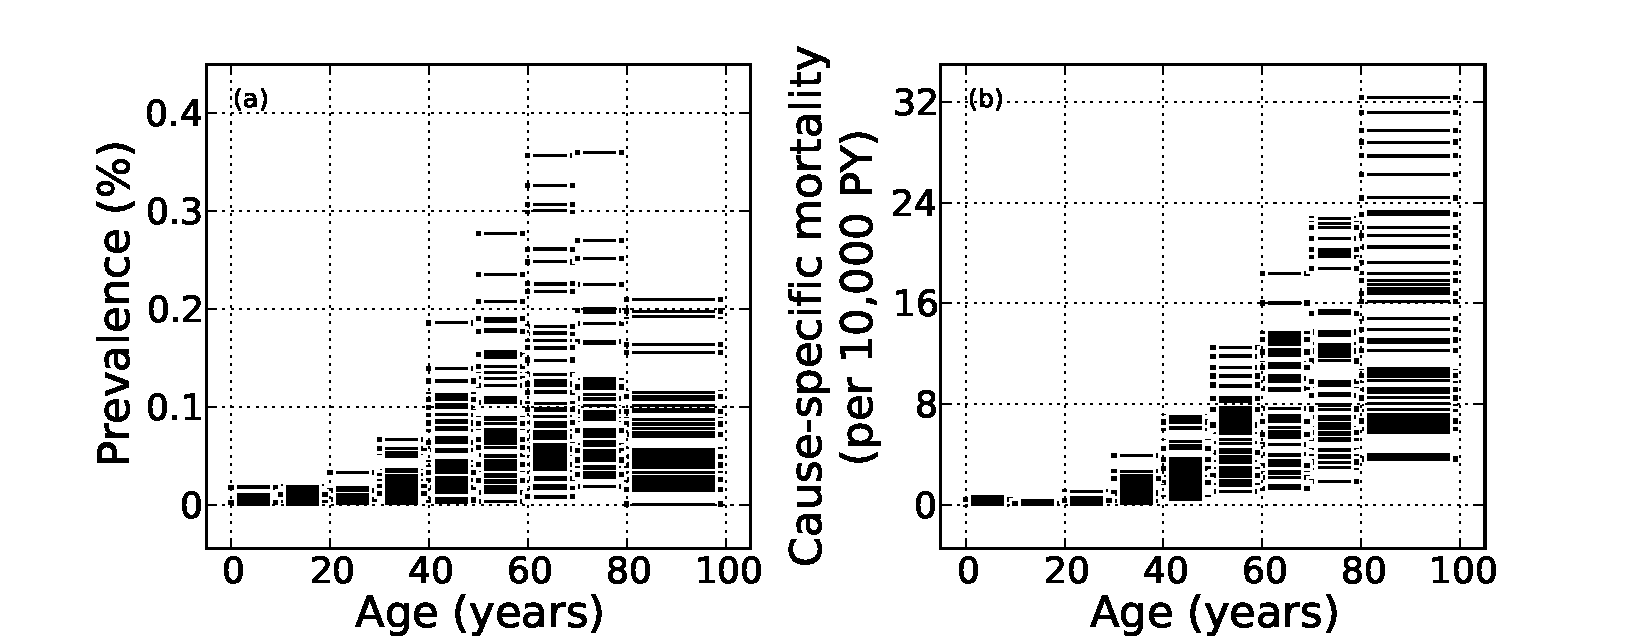
\includegraphics[width=\textwidth]{cirrhosis-data.pdf}
            \caption[Systematic review data for cirrhosis.]{Available 
              global data for cirrhosis (a) prevalence
              and (b) cause-specific mortality.}
            \label{fig:app-cirrhosis data}
        \end{center}
    \end{figure}

Since decompensated cirrhosis is a very severe condition, it is a
sensible hypothesis that there is a strong association between
prevalence and cause-specific mortality rate at the country level.  In
other words, we expected a priori that regions with higher death rates
from cirrhosis would also have higher decompensated cirrhosis prevalence.
Figure~\ref{fig:app-cirrhosis asp} shows the relationship between decompensated cirrhosis
prevalence and the age-standardized death rate (ASDR) of cirrhosis as a
scatterplot, using all data on cirrhosis prevalence collected in
systematic review.

    \begin{figure}[h]
        \begin{center}
            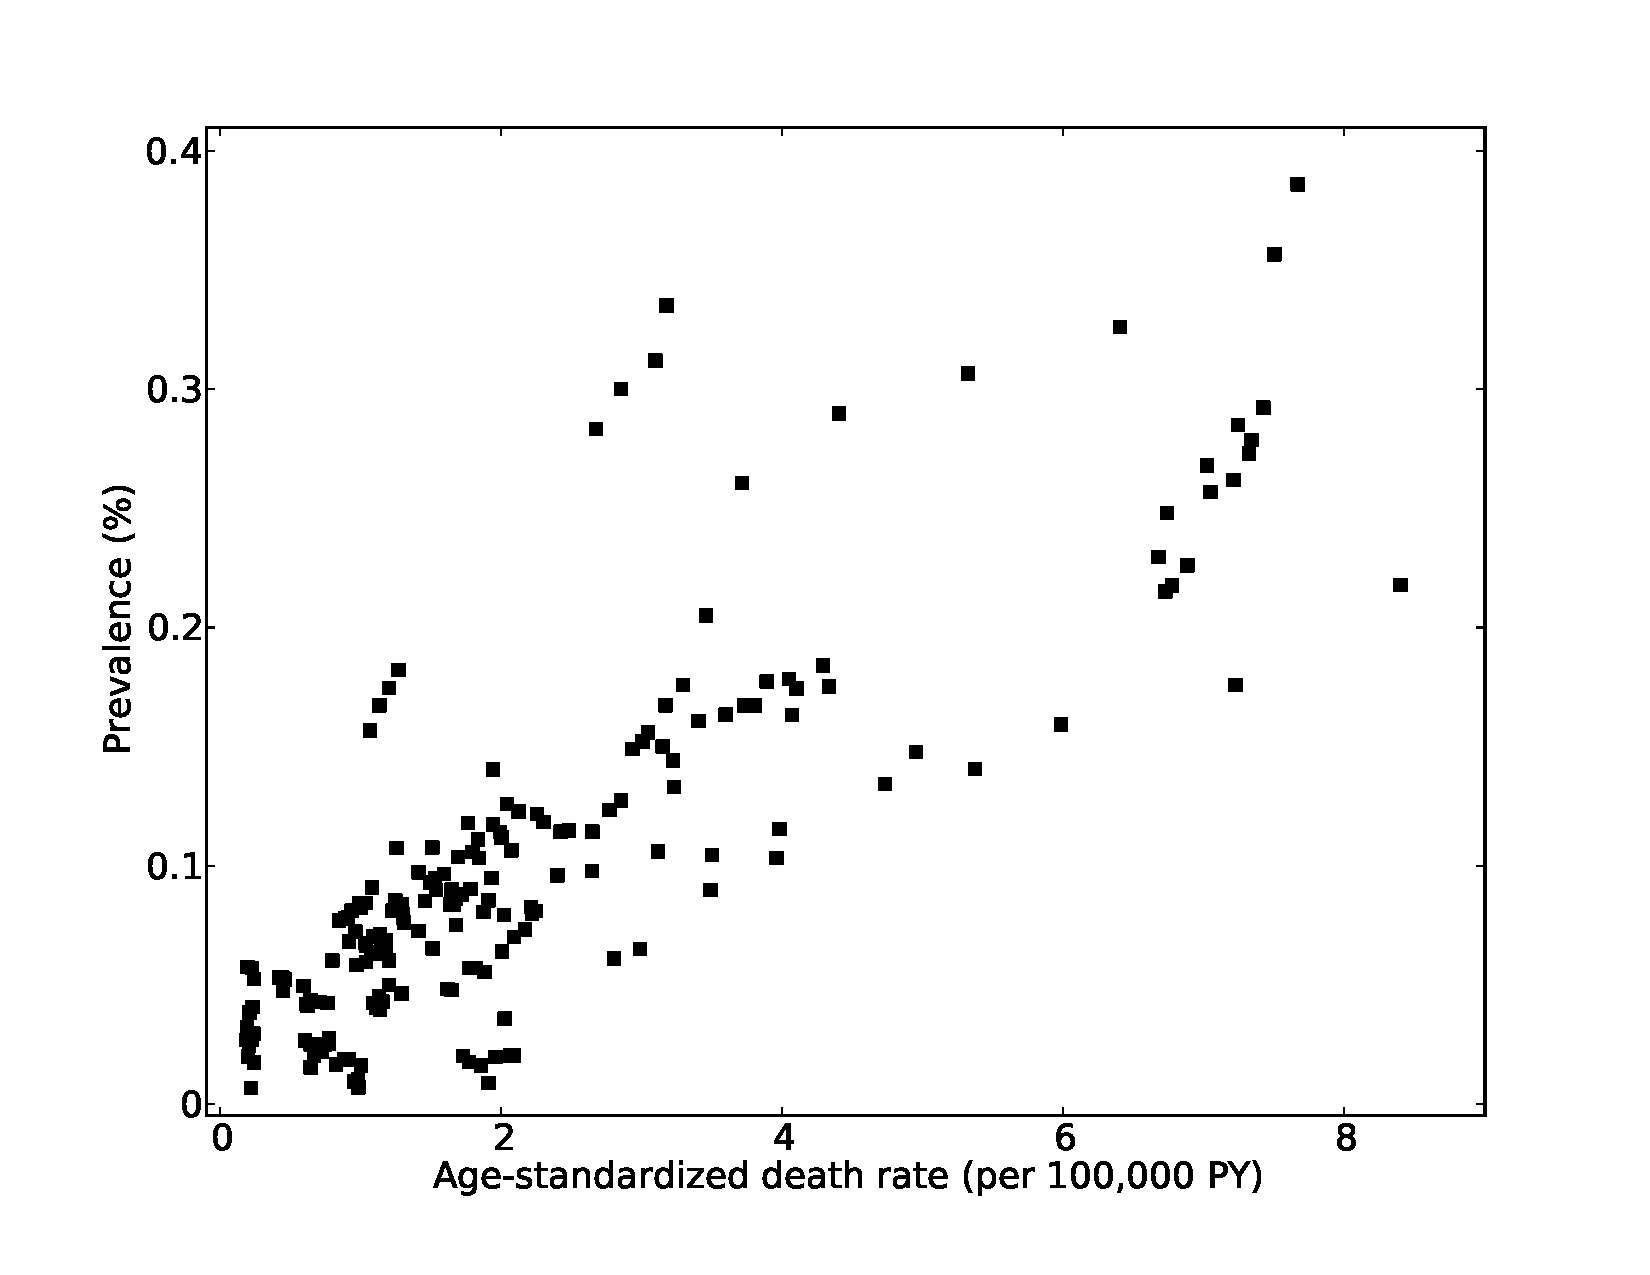
\includegraphics[width=\textwidth]{cirrhosis-lnASDR_v_prev.pdf}
            \caption{Relationship between cirrhosis prevalence data
              collected in systematic review and age-standardized
              death rate of cirrhosis.}
            \label{fig:app-cirrhosis asp}
        \end{center}
    \end{figure}

In regions with no cirrhosis data, estimates of the ASDR
may be used as an explanatory covariate to
estimate cirrhosis prevalence.  By borrowing strength from the
mortality estimates to inform the incidence estimates, cirrhosis
prevalence can be estimated for regions without data as shown in
figure~\ref{fig:app-cirrhosis prev est}.  Since the predictive
covariate fixed effects are modeled as a shift in log-space, it is
often preferable to use the log of the ASDR as
a covariate instead of using the ASDR untransformed.

    \begin{figure}[h]
        \begin{center}
            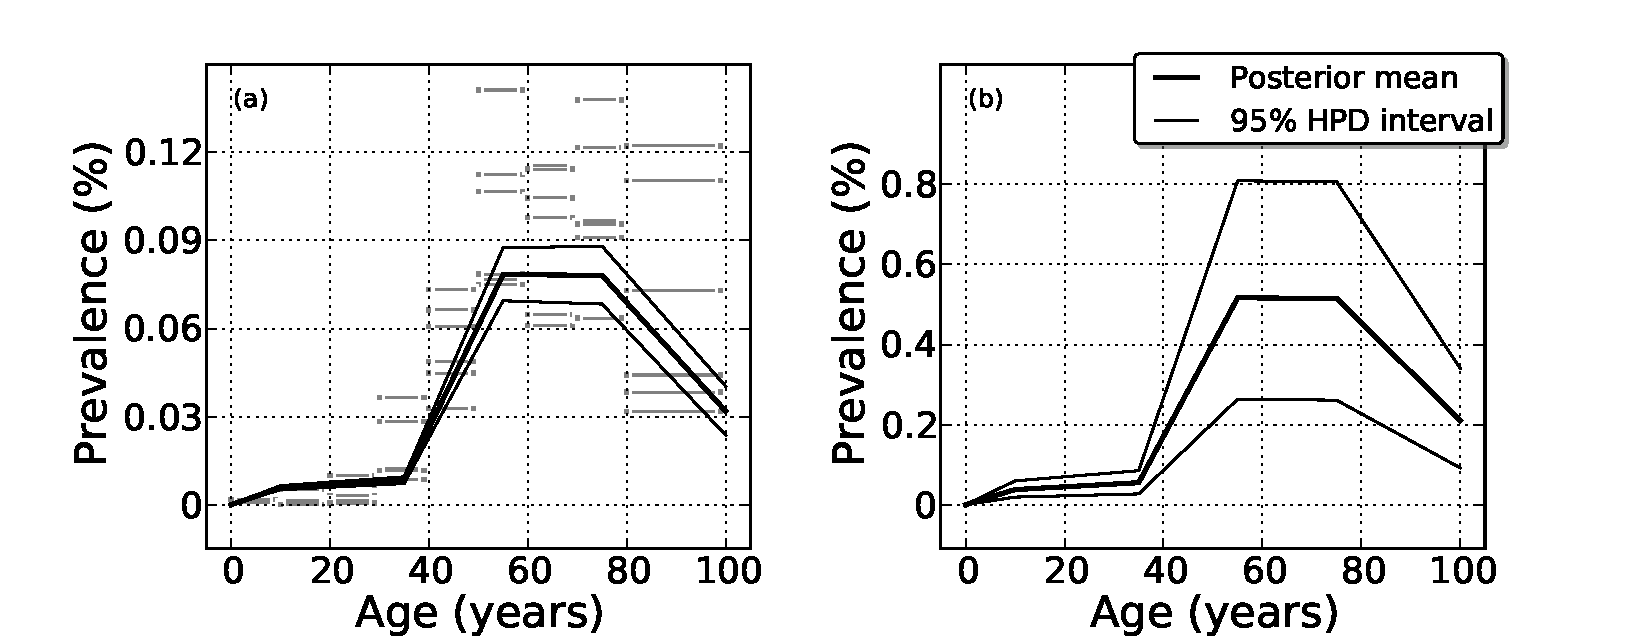
\includegraphics[width=\textwidth]{cirrhosis-prev_est.pdf}
            \caption[Cirrhosis prevalence estimates and available data 
              for the United States of America and Egypt.]{Cirrhosis 
              prevalence estimates and available data
              for (a) the United States of America and (b) Egypt, for males
              in 2005. Note that systematic review found no
              measurements of cirrhosis prevalence for Egypt, and
              prevalence level is extrapolated based on the inferred
              relationship with the age-standardized death rate.}
            \label{fig:app-cirrhosis prev est}
        \end{center}
    \end{figure}

As shown in figure~\ref{fig:app-cirrhosis prev est}(b),
despite the absence of any direct measurements of cirrhosis prevalence
in Egypt, this approach provides a sensible estimate.  It shows that
the prevalence is much higher there than in the United States.  It
also shows a sizable uncertainty interval, reflecting the imperfect
relationship between prevalence and the ASDR.  The age pattern is informed
by borrowing strength from regions like North America where
age-specific data are available.

Even in settings where there is not such a strong explanatory
relationship between the parameter of interest and some covariate,
this approach can still be useful.  Although it would be ideal to have
direct measurements of the quantities of interest, in many cases they
have never been made.  Explaining regional variation with a weak
covariate is preferable to not explaining it at all.
